\section{Difa Al Fansha (1174076)}
\subsection{Instalasi Map Server}
\begin{enumerate}
	\item Download file ms4w-4.0.1-setup.exe di https://ms4w.com/
		\begin{figure}[H]
			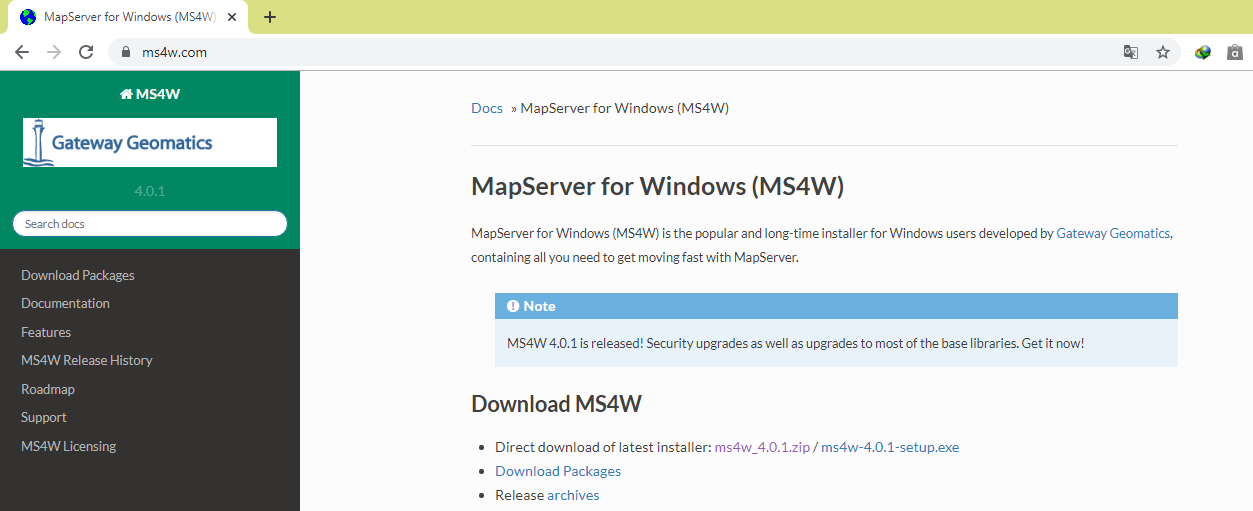
\includegraphics[width=6cm]{figures/Tugas4/1174076/1.png}
			\centering
			\caption{Download installer Map Server}
		\end{figure}
	\item Buka file yang telah di download sebelumnya
		\begin{figure}[H]
			
\includegraphics[width=6cm]{figures/Tugas4/1174076/2.png}
			\centering
			\caption{Menjalankan file ms4w-4.0.1-setup.exe}
		\end{figure}
	\item Klik I Agree, yang artinya kita setuju dengan persyaratan yang diberikan
		\begin{figure}[H]
			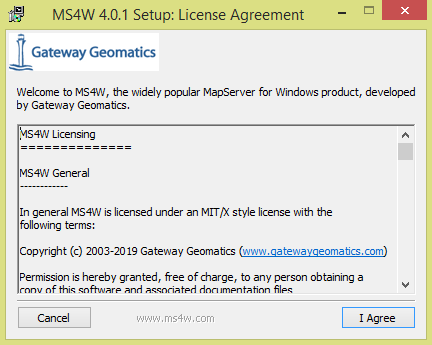
\includegraphics[width=6cm]{figures/Tugas4/1174076/3.png}
			\centering
			\caption{Setuju dengan persyaratan}
		\end{figure}
	\item Lalu pilih komponen apa saja yang akan di install lalu tekan Next
		\begin{figure}[H]
			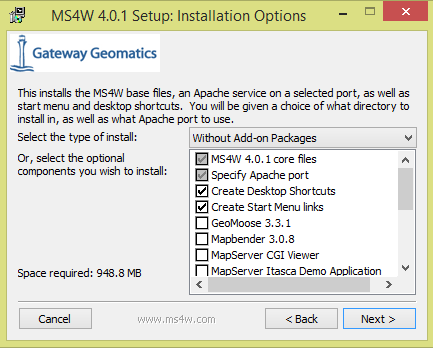
\includegraphics[width=6cm]{figures/Tugas4/1174076/4.png}
			\centering
			\caption{Pilih Komponen yang di install}
		\end{figure}
	\item Pilih di folder mana file akan diinstall, lalu tekan Next
		\begin{figure}[H]
			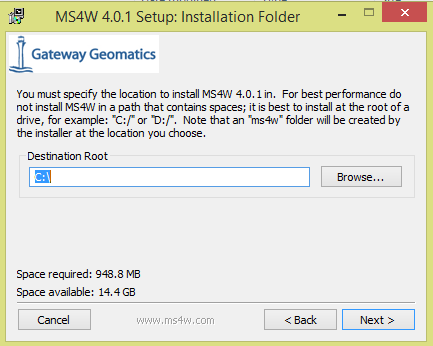
\includegraphics[width=6cm]{figures/Tugas4/1174076/5.png}
			\centering
			\caption{Tentukan path dari file}
		\end{figure}
	\item Pilih port mana yang akan di pakai untuk map server, lalu tekan Next.
	\begin{itemize}
	\item Ketikkan port 8080, sehingga tidak menggangu web server
	\end{itemize}
		\begin{figure}[H]
			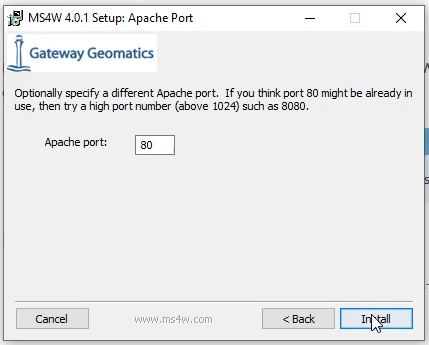
\includegraphics[width=6cm]{figures/Tugas4/1174076/6.png}
			\centering
			\caption{Tentukan port map server}
		\end{figure}
	\item Tekan Yes apabila muncul windows yang akan menginstall vsredist 2017
	\item Tunggu hingga installer berakhir, lalu klik close
		\begin{figure}[H]
			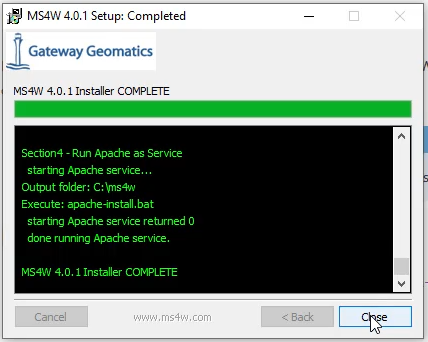
\includegraphics[width=6cm]{figures/Tugas4/1174076/7.png}
			\centering
			\caption{Install selesai}
		\end{figure}
\end{enumerate}

\subsection{Instalasi Map Proxy}
\begin{enumerate}
	\item Buka CMD lalu ketikkan pip install mapproxy 
		\begin{figure}[H]
			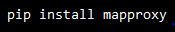
\includegraphics[width=6cm]{figures/Tugas4/1174076/8.png}
			\centering
			\caption{Install Map Proxy}
		\end{figure}
	\item Ketikkan pip install pyproj pada CMD
		\begin{figure}[H]
			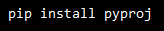
\includegraphics[width=6cm]{figures/Tugas4/1174076/9.png}
			\centering
			\caption{Install Pyproj}
		\end{figure}
\end{enumerate}

\subsection{Konfigurasi Map Server}
\begin{enumerate}
	\item Memastikkan map server berjalan
	\item tekan windows + r, lalu ketikan services.msc seperti yang tertera digambar, lalu tekan OK
		\begin{figure}[H]
			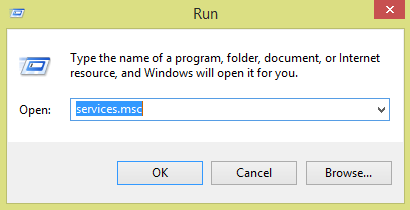
\includegraphics[width=6cm]{figures/Tugas4/1174076/10.png}
			\centering
			\caption{Install Map Proxy}
		\end{figure}
	\item Cari Setting yang bernama Apache MS4W Web Server
	\item Apabila sudah berjalan, gambar akan seperti gambar berikut
		\begin{figure}[H]
			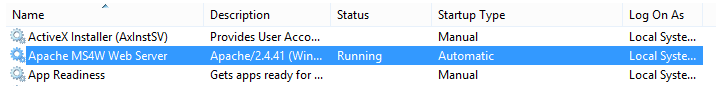
\includegraphics[width=6cm]{figures/Tugas4/1174076/11.png}
			\centering
			\caption{Install Map Proxy}
		\end{figure}
	\item Apabila berbeda, klik 2 kali Apache MS4W lalu Ubah startup ke Automatic, seperti gambar berikut
		\begin{figure}[H]
			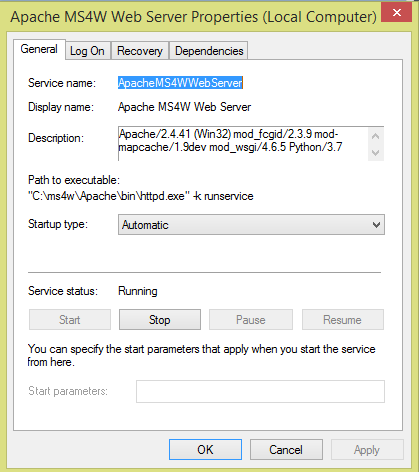
\includegraphics[width=6cm]{figures/Tugas4/1174076/12.png}
			\centering
			\caption{Install Map Proxy}
		\end{figure}
\end{enumerate}

\subsection{Pengujian}
\begin{enumerate}
	\item Download github di https://github.com/awangga/gede
	\item lalu ekstrak file yang di download
	\item Buka file shp
	\item lalu buka file 0.shp dengan QGIS
		\begin{figure}[H]
			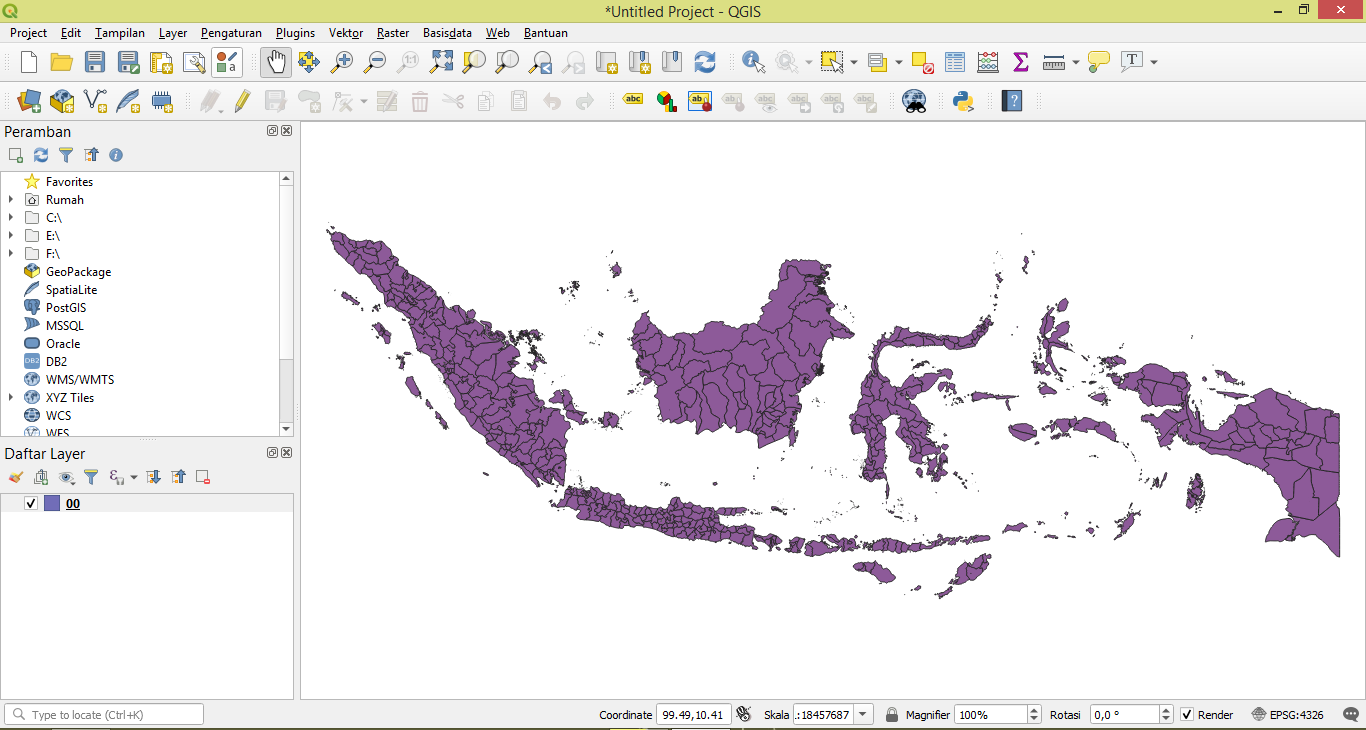
\includegraphics[width=6cm]{figures/Tugas4/1174076/13.png}
			\centering
			\caption{Install Map Proxy}
		\end{figure}
\end{enumerate}


\subsection{Link install Map Server}
https://youtu.be/DrrXcLo320w
\subsection{Menampilkan Map Indonesia dengan QGIS}
https://youtu.be/m3zRxbm69VU
